\documentclass{article}

\PassOptionsToPackage{numbers, sort&compress}{natbib}
\usepackage[final]{neurips_2019}
\usepackage[utf8]{inputenc}
\usepackage[T1]{fontenc}
\usepackage{hyperref}
\usepackage{url}
\usepackage{booktabs}
\usepackage{amsfonts}
\usepackage{amsmath}
\usepackage{amssymb}
\usepackage{nicefrac}
\usepackage{microtype}
\usepackage{graphicx}
\usepackage{subcaption}
\usepackage{xcolor}
\usepackage{placeins}
\usepackage{float}

\graphicspath{{figures/}}
\setlength{\tabcolsep}{3.5pt}
\renewcommand{\arraystretch}{1.02}
\setlength{\textfloatsep}{8pt}
\setlength{\floatsep}{6pt}
\setlength{\intextsep}{6pt}
\setlength{\abovecaptionskip}{3pt}
\setlength{\belowcaptionskip}{2pt}
\setcounter{topnumber}{4}
\setcounter{bottomnumber}{3}
\setcounter{totalnumber}{6}
\renewcommand{\topfraction}{0.92}
\renewcommand{\bottomfraction}{0.8}
\renewcommand{\textfraction}{0.08}
\renewcommand{\floatpagefraction}{0.85}
\newcommand{\pend}[1]{\textcolor{red}{[#1]}}
\makeatletter
\renewcommand{\@notice}{}
\makeatother

\title{Adapting, Connecting and Sampling from Language Models: \\
  Fine-Tuning Trade-Offs, Visual Grounding and Test-Time Compute}
\author{%
  Muhammad Umair \\
  Lahore University of Management Sciences \\
  \texttt{25280013@lums.edu.pk}
}

\begin{document}
\maketitle

\begin{abstract}
We report three experiments on getting more out of small language models. First, we fine-tune Qwen3-0.6B on 40,000 MetaMathQA examples with full fine-tuning, L2-SP, LoRA and OPLoRA. All five runs raise GSM8K by 16.5 to 21.9 points over the 43.1\% baseline; their clearest differences are off-target, where unrestricted training loses 1.4 points on HellaSwag and shifts BoolQ answers towards ``no'', and where OPLoRA's exact subspace protection gives no measurable benefit over plain LoRA at matched rank. Second, we connect a frozen SigLIP encoder to frozen Qwen through a trained connector and LoRA adapters. On held-out complementary pairs, swapping in the partner image lowers accuracy by 58.6 points on annotation-derived questions and 22.2 points on VQAv2, and 49 visual tokens show no measurable loss against 196 at less than half the training time. Third, on 64,000 supplied Qwen2.5 rollouts we separate sampling failures from selection failures. At 32 candidates, a correct answer exists for about 90\% of questions, but the best rule returns one for 75.7\% (MATH) and 64.6\% (MathVista). Mean log-probability gets worse with more samples and at 32 candidates returns capped rollouts roughly ten times more often than their base rate, while agreement-based stopping keeps fixed-32 accuracy within interval at about half the tokens. Code, configurations, split IDs and results: \url{https://github.com/umairs5/atml-pa3}.
\end{abstract}

\section{Introduction}
Fine-tuning, connecting a vision encoder and spending more compute at inference are three cheap ways of extending a pretrained model. Each has an obvious measure of success and a less obvious cost: a fine-tuned model can gain on its target and lose elsewhere, a vision-language model can answer well from language priors, and more samples can produce a correct answer that the selection rule then fails to pick. We therefore compare methods against controls designed to expose those costs: benchmarks away from the training domain, complementary image pairs, and oracle coverage. Each task below uses seed 6304. All GPU runs used one Colab T4.

\section{Task 1: Large language model fine-tuning}
\paragraph{Setup.} All runs start from \texttt{Qwen/Qwen3-0.6B} \citep{yang2025qwen3} with thinking disabled and train for one epoch on the first 40,000 eligible MetaMathQA examples \citep{yu2023metamath} (1,250 updates, effective batch 32). Full FT uses a peak learning rate of $2\times10^{-5}$; L2-SP \citep{li2018l2sp} adds a starting-point penalty with $\lambda=10^{-3}$; LoRA \citep{hu2022lora} uses $(r,\alpha)=(4,8)$ and $(16,32)$ at $2\times10^{-4}$ on all seven projection types; OPLoRA \citep{xiong2025oplora} uses $r=16$, $k=128$ and the same initial factors as LoRA-16. We evaluate the unchanged model, Full FT at its midpoint, and the five final models with lm-evaluation-harness 0.4.13 \citep{lmeval}: GSM8K \citep{cobbe2021gsm8k} measures transfer, and HellaSwag \citep{zellers2019hellaswag}, BoolQ \citep{clark2019boolq} and ARC-Easy \citep{clark2018arc} probe retention. Pairwise comparisons use a question-level paired bootstrap (10,000 resamples) and exact McNemar tests, Holm-adjusted over 48 comparisons. All conclusions rest on one seed.

\begin{table}[t]
\centering\small
\caption{Primary scores (\%) and change from the baseline in percentage points. GSM8K uses flexible-extraction exact match; HellaSwag and ARC-Easy normalized accuracy; BoolQ accuracy (majority class 62.2\%).}
\label{tab:t1}
\begin{tabular}{lcccc}
\toprule
Condition & GSM8K & HellaSwag & BoolQ & ARC-Easy \\
\midrule
Baseline & 43.14 & 47.30 & 64.43 & 56.02 \\
Full FT (mid) & 56.79 (+13.65) & 45.43 (-1.87) & 61.83 (-2.60) & 62.12 (+6.10) \\
Full FT & 63.76 (+20.62) & 45.87 (-1.43) & 61.50 (-2.94) & 63.64 (+7.62) \\
L2-SP & 65.05 (+21.91) & 46.34 (-0.97) & 68.26 (+3.82) & 63.01 (+6.99) \\
LoRA-4 & 59.67 (+16.53) & 47.38 (+0.08) & 66.64 (+2.20) & 63.30 (+7.28) \\
LoRA-16 & 61.41 (+18.27) & 47.45 (+0.15) & 72.32 (+7.89) & 63.93 (+7.91) \\
OPLoRA-16 & 61.56 (+18.42) & 47.23 (-0.07) & 72.51 (+8.07) & 63.55 (+7.53) \\
\bottomrule
\end{tabular}
\end{table}

\begin{table}[t]
\centering\footnotesize
\caption{Paired differences in points at the final checkpoints, with 95\% bootstrap intervals. $^{*}$: Holm-adjusted McNemar $p<0.05$.}
\label{tab:t1tests}
\begin{tabular}{lcccc}
\toprule
Comparison & GSM8K & HellaSwag & BoolQ & ARC-Easy \\
\midrule
L2-SP $-$ Full FT & +1.3 [-0.5, +3.1] & +0.5 [+0.1, +0.8] & +6.8 [+5.5, +8.0]$^{*}$ & -0.6 [-1.6, +0.3] \\
LoRA-16 $-$ LoRA-4 & +1.7 [-0.2, +3.7] & +0.1 [-0.3, +0.4] & +5.7 [+4.3, +7.1]$^{*}$ & +0.6 [-0.3, +1.6] \\
OPLoRA-16 $-$ LoRA-16 & +0.2 [-1.4, +1.7] & -0.2 [-0.5, +0.0] & +0.2 [-0.5, +0.8] & -0.4 [-1.0, +0.3] \\
LoRA-16 $-$ Full FT & -2.4 [-4.6, -0.1] & +1.6 [+1.1, +2.1]$^{*}$ & +10.8 [+9.0, +12.7]$^{*}$ & +0.3 [-0.9, +1.4] \\
\bottomrule
\end{tabular}
\end{table}

\paragraph{Specialization and retention.} Table~\ref{tab:t1} shows that every method improves GSM8K and ARC-Easy significantly, so mathematical training transfers to elementary science as well as to word problems. Full FT keeps improving through training: the final model beats its own midpoint by 7.0 points on GSM8K [4.5, 9.4] and 1.5 on ARC-Easy, although 94\% of its final displacement ($\|\theta-\theta_0\|_2$ of 10.02 against 10.65) is already reached at the midpoint. Loss on HellaSwag is real but small. Full FT loses 1.4 points and L2-SP 1.0, both significant against the baseline, whereas no LoRA variant moves by more than 0.15. This agrees with the finding of \citet{biderman2024lora} that LoRA forgets less, though here the gap to Full FT is 1.6 points rather than a collapse.

BoolQ looks like forgetting under Full FT ($-$2.9 points), but the predictions tell a different story. The share of ``yes'' answers falls from 57.8\% to 31.3\%: accuracy on true-yes questions drops from 67.9\% to 44.2\% while accuracy on true-no questions rises from 58.8\% to 89.9\%. So this is largely a shift in decision bias, and a single accuracy figure hides it. LoRA-16's +7.9 is different in kind, since it improves both classes (76.8\% and 64.9\%) at a yes-rate of 61.0\%, close to the true 62.2\%. We did not expect an off-target gain of this size and cannot explain it from these measurements.

\paragraph{Restrictions on adaptation.} Table~\ref{tab:t1tests} gives the controlled comparisons. L2-SP reduces final displacement by 41\% (6.28 against 10.65), with a penalty term $\lambda\Omega$ of about 0.02 against an SFT loss near 0.18 (Figure~\ref{fig:t1}), and costs nothing detectable on GSM8K. Its BoolQ gain over Full FT is large, while its HellaSwag gain does not survive correction. Quadrupling LoRA rank does not significantly raise GSM8K (+1.7 [$-$0.2, 3.7]) but does raise BoolQ. Full FT's GSM8K lead over LoRA-16 (2.4 points) has an interval that just excludes zero and does not survive correction, so we do not claim a difference. The clear GSM8K gap is between the extremes: L2-SP beats LoRA-4 by 5.4 points [3.0, 7.8]. OPLoRA is the clearest null: at matched rank and initialization, it differs from LoRA-16 by at most 0.4 points on every benchmark, none significant. This does not show the two are equivalent, only that any difference is below what these sample sizes detect.

\begin{figure}[t]
\centering
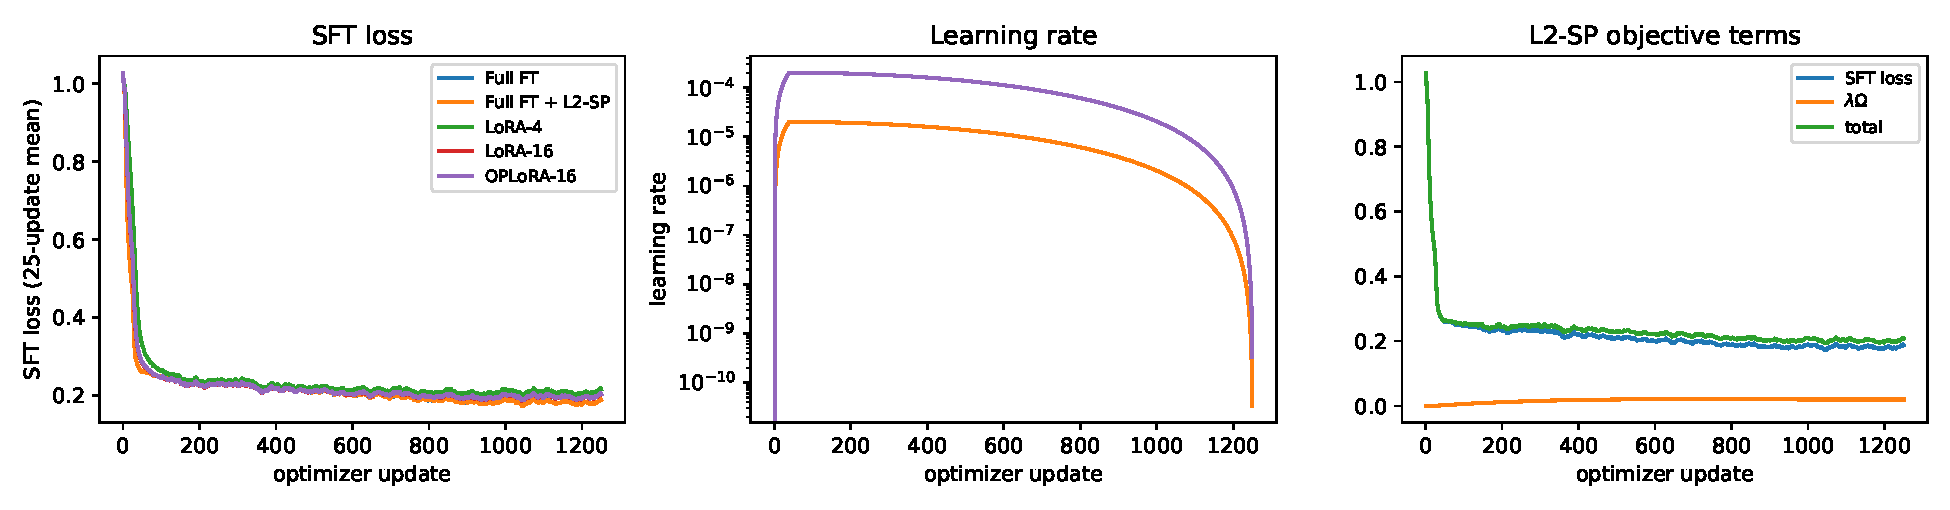
\includegraphics[width=\linewidth]{task1_curves.pdf}
\caption{SFT loss (Full FT lies under L2-SP; LoRA-16 under OPLoRA-16), learning rate, and the L2-SP objective.}
\label{fig:t1}
\end{figure}

\begin{table}[t]
\centering\footnotesize
\caption{\texttt{down\_proj} diagnostics at layers 0/13/27: subspace interference $\rho_k$, relative update size $\eta$, and the ratio of mean correction $R(z)$ on math over non-math probes.}
\label{tab:t1diag}
\begin{tabular}{lccccccccc}
\toprule
 & \multicolumn{3}{c}{$\rho_k$} & \multicolumn{3}{c}{$\eta$} & \multicolumn{3}{c}{$R$ math / non-math} \\
Condition & L0 & L13 & L27 & L0 & L13 & L27 & L0 & L13 & L27 \\
\midrule
Full FT (mid) & 0.132 & 0.148 & 0.116 & 0.0134 & 0.0154 & 0.0125 & 3.9 & 3.4 & 0.5 \\
Full FT & 0.132 & 0.148 & 0.115 & 0.0138 & 0.0160 & 0.0130 & 3.9 & 3.3 & 0.5 \\
L2-SP & 0.133 & 0.150 & 0.107 & 0.0112 & 0.0137 & 0.0079 & 3.9 & 2.9 & 0.5 \\
LoRA-4 & 0.135 & 0.140 & 0.105 & 0.0093 & 0.0101 & 0.0068 & 17.1 & 40.8 & 0.6 \\
LoRA-16 & 0.145 & 0.141 & 0.116 & 0.0148 & 0.0183 & 0.0115 & 2.2 & 4.9 & 0.5 \\
OPLoRA-16 & 0.000 & 0.000 & 0.000 & 0.0147 & 0.0188 & 0.0094 & 2.3 & 4.6 & 0.5 \\
\bottomrule
\end{tabular}
\end{table}

\paragraph{Parameter changes and behavior.} Table~\ref{tab:t1diag} confirms that the OPLoRA constraint holds: $\rho_k$ is zero to within $4\times10^{-8}$ at all three layers, against 0.11 to 0.15 elsewhere, at a similar $\eta$. Yet removing that interference changes no benchmark measurably, so at these update sizes ($\eta$ under 2\%) the overlap with leading singular directions does not appear to be what limits retention. The activation ratios show that corrections respond more to math prompts at layers 0 and 13 (41-fold for LoRA-4 at layer 13) and the reverse at layer 27. Low rank appears to give the most selective corrections. These are correlations at three sampled layers of one module type: they do not establish that any update causes a benchmark change, and $\rho_k$ on \texttt{down\_proj} says nothing about the rest of the network.

\begin{table}[t]
\centering\footnotesize
\begin{minipage}{0.46\linewidth}\centering
\caption{Resources for the five runs. Times and memory on a T4; checkpoint is the final recovery state.}
\label{tab:t1res}
\begin{tabular}{lcccc}
\toprule
Run & Params (M) & Min & GB & Ckpt \\
\midrule
Full FT & 596.05 & 140 & 11.69 & 8.9G \\
L2-SP & 596.05 & 146 & 11.69 & 8.9G \\
LoRA-4 & 2.52 & 162 & 3.14 & 40M \\
LoRA-16 & 10.09 & 158 & 3.26 & 155M \\
OPLoRA-16 & 10.09 & 207 & 3.56 & 155M \\
\bottomrule
\end{tabular}
\end{minipage}\hfill
\begin{minipage}{0.51\linewidth}\centering
\caption{Annotation of the 42 fixed responses (6 per condition): format met, coherent (yes+partial), repetition, maths framing, inappropriate, truncated.}
\label{tab:t1ann}
\begin{tabular}{lcccccc}
\toprule
 & Fmt & Coh. & Rep. & Math & Inap. & Trunc. \\
\midrule
Baseline & 3 & 3+0 & 0 & 0 & 0 & 0 \\
Full FT (mid) & 3 & 0+3 & 2 & 3 & 0 & 2 \\
Full FT & 4 & 1+3 & 1 & 3 & 0 & 1 \\
L2-SP & 4 & 2+2 & 1 & 2 & 0 & 1 \\
LoRA-4 & 5 & 3+2 & 0 & 0 & 0 & 0 \\
LoRA-16 & 4 & 2+2 & 1 & 2 & 0 & 1 \\
OPLoRA-16 & 3 & 3+1 & 2 & 2 & 0 & 0 \\
\bottomrule
\end{tabular}
\end{minipage}
\end{table}

\paragraph{Cost and behavior beyond benchmarks.} Table~\ref{tab:t1res} shows the practical difference: LoRA checkpoints are 40 to 155\,MB against 8.9\,GB. The full runs take 140 and 146 minutes at 11.7\,GB peak allocation; L2-SP's penalty adds 6 minutes and keeps its 2.4\,GB reference on the CPU. The LoRA runs need 3.1 to 3.6\,GB but save memory rather than time here (158 and 162 minutes on shared Colab GPUs, so small timing gaps are not meaningful). OPLoRA-16 takes 31\% longer than LoRA-16 (207 minutes) and holds a 323\,MB projection basis from a 34\,s SVD, while its exported adapter is the same size as LoRA-16's. The annotated subset covers the first and last plain questions in the file (\emph{what is your wish}, \emph{enough of my husband}) in all three formats. Mathematical framing is the clearest behavioral change: the baseline never does it, but 12 of the 36 fine-tuned responses add a line such as ``The answer is: 1'', including after a sound answer about a marriage (LoRA-16 and OPLoRA-16). Repetition to the 512-token cap affects Full FT (midpoint and final), L2-SP and LoRA-16, for example Full FT's ``If you're still feeling overwhelmed, it's important to take a break'', while the baseline gives a short reply. LoRA-4 has the cleanest record. JSON is a weak point for all: no model produced parseable JSON on the second question, and the baseline's code fences fail the strict check. We found no inappropriate content, but 42 responses cannot establish its absence. We chose these excerpts because they are the same question and format across conditions.

\section{Task 2: Vision-language model and visual grounding}
\paragraph{Setup.} We cache the 196 final patch features of a frozen SigLIP encoder \citep{zhai2023siglip} in FP16, map them through a two-layer connector \citep{liu2023llava} with a fixed calibrated output scale (0.055 for 196 tokens, matching visual and text embedding norms at initialization), and insert them into a frozen Qwen prompt. Training has three stages: caption alignment (2,250 updates, connector only), visual instruction (1,500 updates, adding LoRA $r=16$ on \texttt{q/k/v/o} projections; presence, counting and caption draws at 50/25/25\%), and natural VQA (750 updates; VQAv2 70\% with 10\% each of replay). Data come from COCO 2014 \citep{lin2014coco} and VQAv2 complementary pairs \citep{goyal2017vqa} with consensus of at least 8 of 10 annotators. Our checks found zero image overlap between training and evaluation and among evaluation sets, and rerunning the selection reproduces the files exactly. We evaluate on 64 grounding and 96 VQAv2 test pairs under four image conditions. Intervals come from 4,000 pair-level bootstrap resamples.

\begin{figure}[t]
\centering
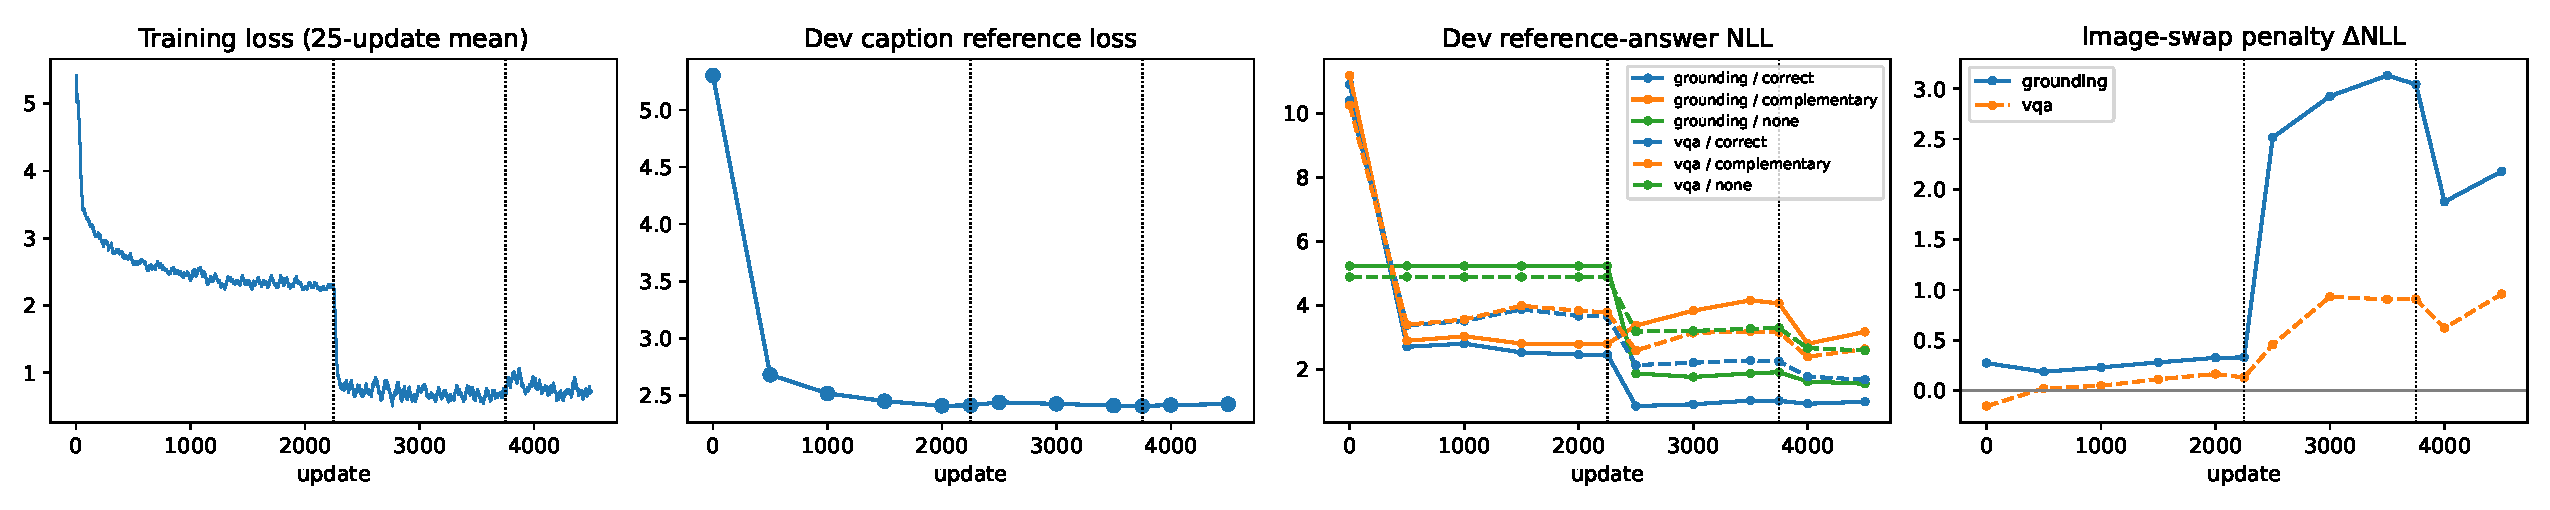
\includegraphics[width=\linewidth]{task2_curves.pdf}
\caption{Training and development curves for the 196-token model; dotted lines mark stage boundaries.}
\label{fig:t2}
\end{figure}

\paragraph{Learning a visual interface.} Figure~\ref{fig:t2} shows what each stage contributes. Caption alignment halves development caption loss (5.30 to 2.41), and that loss stays between 2.40 and 2.44 in later stages, so no forgetting of captioning is visible. But it teaches little grounding: after Stage 1, development grounding accuracy is 22.9\% with the correct image and the same with an unrelated one, and VQAv2 is no better with the correct image than the swapped one (26.6\% against 28.9\%). Stage 2 is where the model starts using images: the grounding swap penalty jumps from 0.33 to 3.04 nats and accuracy reaches 70.8\%. VQAv2 also improves to 52.7\%, with a swap penalty of 0.91, before seeing any VQA training data. Stage 3 trades some of this: VQAv2 rises to 56.3\% while grounding falls to 60.4\% and its swap penalty to 2.18, with grounding replay at only 20\% of draws. On 24 development grounding pairs that drop is imprecise. No-image NLL also falls across stages (5.23, 1.92 and 1.55 on grounding at the stage ends), which shows that adapters also teach the answer format and priors without any image.

\begin{table}[t]
\centering\footnotesize
\caption{Final test results (Stage 3). Accuracy with 95\% interval; pair: both sides correct; same: both sides give one answer; partner: answer follows the partner's reference; NLL of references (for the difference row, compl. minus correct).}
\label{tab:t2}
\begin{tabular}{lcccccc}
\toprule
Image condition & Accuracy (196) & Pair & Same & Partner & NLL & Acc. (49) \\
\midrule
\multicolumn{7}{l}{\emph{Grounding (64 pairs)}} \\
Correct & 69.5 [60.9, 78.1] & 50.0 & 20.3 & 10.9 & 0.71 & 74.2 \\
Complementary & 10.9 [6.2, 16.4] & 0.0 & 20.3 & 69.5 & 3.29 & 9.4 \\
Mismatched & 32.8 [26.6, 39.1] & 1.6 & 70.3 & 38.3 & 2.29 & 34.4 \\
No image & 37.5 [32.0, 42.2] & 0.0 & 100.0 & 37.5 & 1.52 & 36.7 \\
Correct $-$ compl. & +58.6 [+46.9, +70.3] & & & & +2.58 & +64.8 \\
\multicolumn{7}{l}{\emph{VQAv2 (96 pairs)}} \\
Correct & 50.4 [43.5, 57.2] & 21.9 & 50.0 & 25.0 & 1.66 & 47.1 \\
Complementary & 28.1 [22.4, 33.5] & 2.1 & 50.0 & 47.4 & 2.50 & 24.8 \\
Mismatched & 31.6 [26.2, 37.1] & 1.0 & 72.9 & 30.2 & 2.52 & 30.4 \\
No image & 27.9 [22.6, 33.3] & 0.0 & 100.0 & 25.5 & 2.72 & 33.0 \\
Correct $-$ compl. & +22.2 [+13.2, +31.4] & & & & +0.84 & +22.3 \\
\bottomrule
\end{tabular}
\end{table}

\begin{figure}[t]
\centering
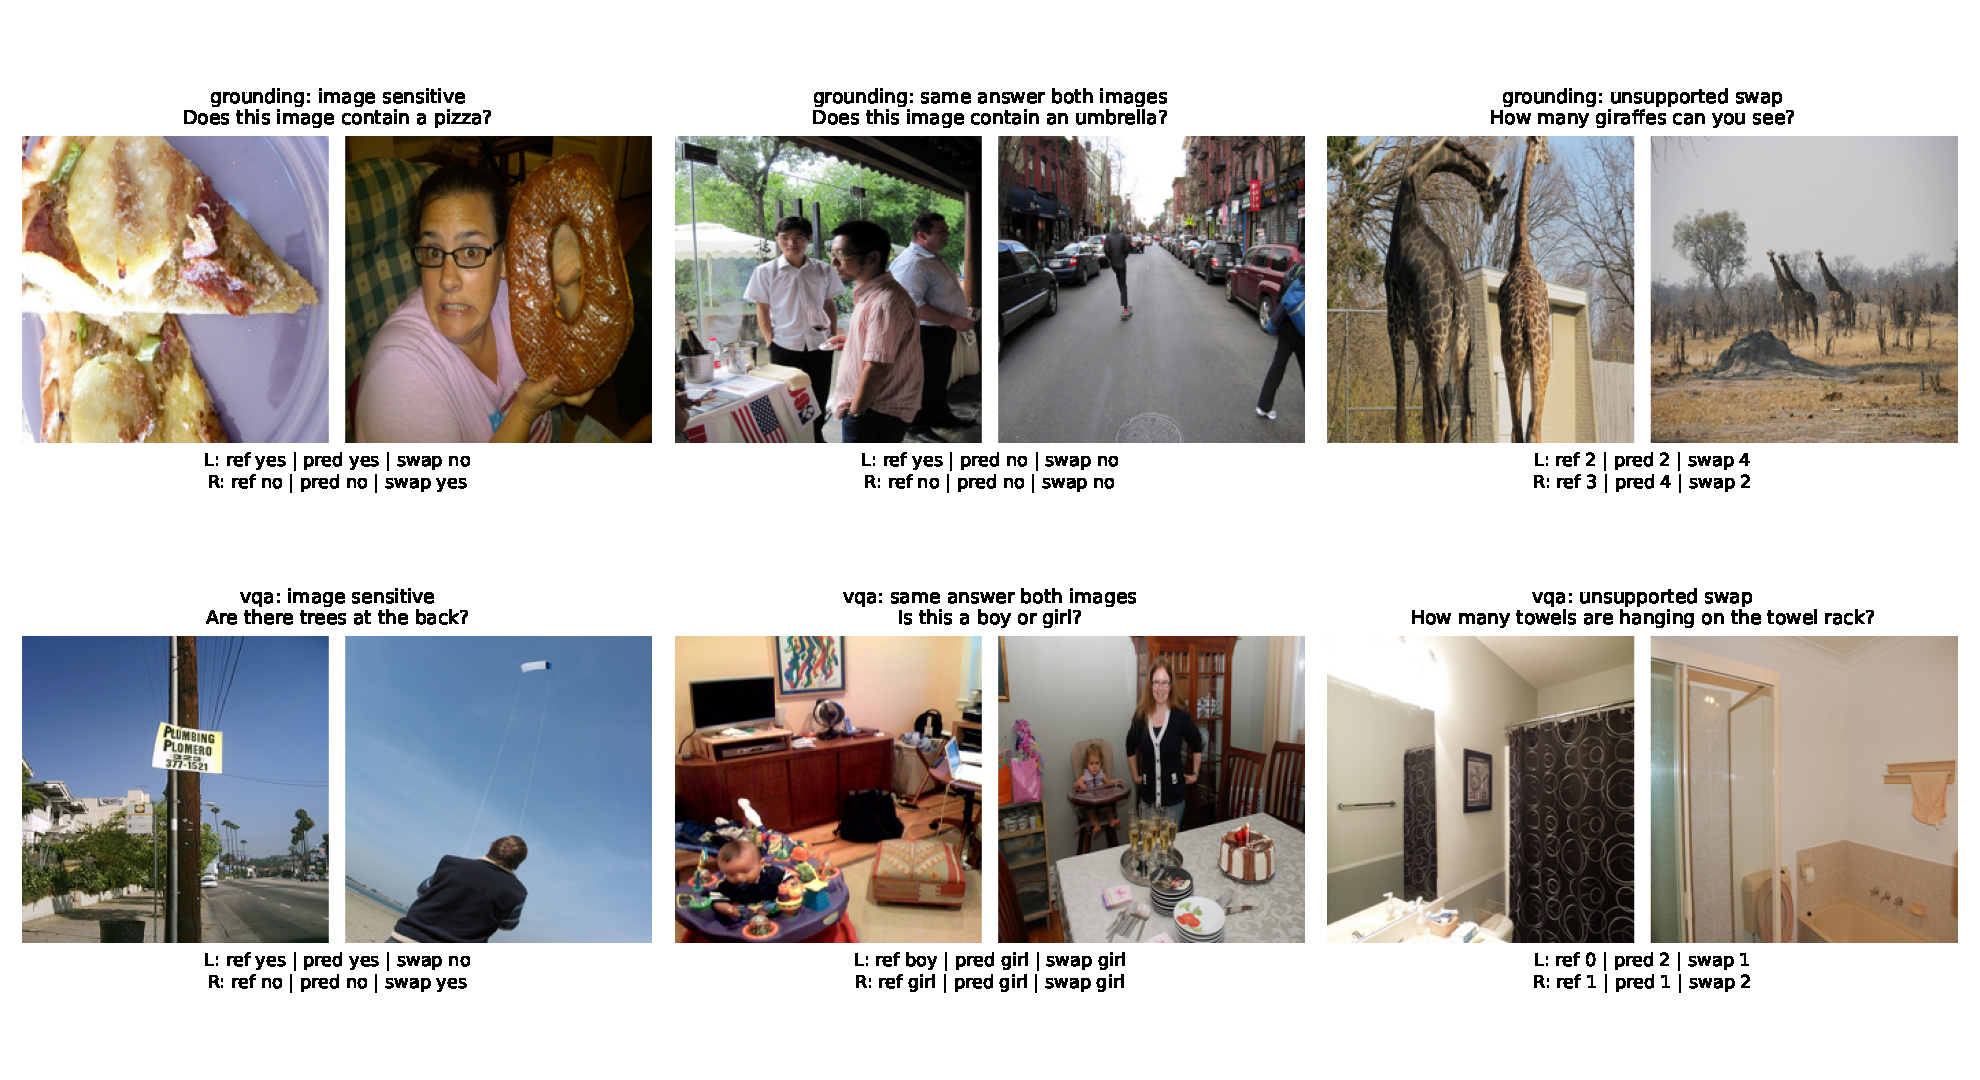
\includegraphics[width=0.86\linewidth]{task2_examples.pdf}
\caption{Aligned complementary pairs (196 tokens), with the first pair of each class in a seed-6304 shuffle: image-sensitive, same answer on both images, and unsupported swap. L/R: left and right image; swap: prediction when shown the other image. A further pair per class is saved in the repository.}
\label{fig:t2ex}
\end{figure}

\paragraph{Grounding and generalization.} Table~\ref{tab:t2} gives the central result. A model that ignored images would score the same with the correct and complementary image, since each pair shares its question. Instead accuracy falls from 69.5\% to 10.9\% on grounding and from 50.4\% to 28.1\% on VQAv2, and both intervals exclude zero by a wide margin. The fall is not just damage. Under a swap, answers follow the partner's reference for 69.5\% of grounding questions and 47.4\% of VQAv2 questions, so on grounding the model usually answers from what it sees, and on VQAv2 the partner's answer is the most common outcome without being a majority. About a fifth of grounding swaps (19.5\%) and 27.6\% of VQAv2 swaps match neither side. Grounding is unevenly learned. Presence reaches 95.3\% against a 50\% no-image level, whereas counting reaches 43.8\% (Appendix~\ref{app:t2}), with COCO's annotation noise as one possible contributor. VQAv2 is further from reliable: both sides of a pair receive one answer in 50\% of pairs, and only 21.9\% have both sides right. Its no-image accuracy of 27.9\% also shows how much language priors offer. Figure~\ref{fig:t2ex} illustrates these classes, including counting errors where the model changes answer but to an unsupported value.

\paragraph{Measuring image use and cost.} Likelihood and generation agree on direction: the NLL advantage over the complementary image is 2.58 nats on grounding and 0.84 on VQAv2. Pair metrics add what neither shows, namely that VQAv2's advantage rests on few fully correct pairs. On grounding, wrong images hurt more than no image in NLL (3.29 and 2.29 against 1.52), although the no-image input also has a shorter prefix; on VQAv2 the order reverses (2.50 and 2.52 against 2.72). Captions are generic but scene-appropriate (``A kitchen with a stove and a sink.''), and sometimes garble specifics (``A horseman is holding a banner with a picture of a horse.'' for a woman with a flag). Feature caching took 122\,s (76 images/s, 1.73\,GB peak, 2.79\,GB stored) for 9,277 images. Training has 1.84M trainable parameters in Stage 1 and 6.42M in Stages 2 and 3, and took 103 minutes at 1.56\,GB peak allocation with six updates skipped by the loss scaler. Generation costs 41\,ms per answer. The optional 49-token run takes 45 minutes and 22\,ms per answer at 1.48\,GB. Its correct-image differences from the 196-token model cross zero on both suites (+4.7 [$-$2.3, 11.7] on grounding, $-$3.3 [$-$9.8, 3.1] on VQAv2), so we find no measurable loss from pooling at this test size. Its one clear accuracy difference is no-image VQAv2 (+5.2 [1.3, 9.1]), which involves no visual input at all and likely reflects the separately trained adapters.

\section{Task 3: Test-time compute}
\paragraph{Setup.} We use the supplied 32 rollouts per question from Qwen2.5-3B on 1,000 MATH questions \citep{qwen2024qwen25,hendrycks2021math} and Qwen2.5-VL-3B on 1,000 MathVista questions \citep{bai2025qwen25vl,lu2024mathvista}; token lists align with their counts in all 64,000 rollouts. Following the prescribed permutation, 200 questions form the development set and 800 the held-out set, on which all accuracy and cost figures are reported. (MATH's development set happens to be easier: fixed-32 accuracy is 83.0\% against 74.0\%, so splits should not be compared.) Answers are grouped without gold labels and graded with the same rule: math-verify 0.9.0 \citep{mathverify} for MATH, and MathVista's answer-type, choice and precision rules with its option letters, after removing LaTeX units. Missing extractions form one NO\_ANSWER group that always counts as wrong (521 and 3,032 rollouts across all 1,000 questions). A further 1,322 MathVista answers do not parse under their question type; they vote as their own groups but cannot be correct. Forty MATH comparisons with enormous exponents hit a 5\,s limit and count as not equivalent. Each budget $N\in\{1,2,4,8,16,32\}$ uses ten saved orders, with intervals from 1,000 paired question-level resamples. Self-certainty, VisConf and RWC follow \citet{kang2025selfcertainty} and \citet{usman2026visconf}.

\begin{figure}[t]
\centering
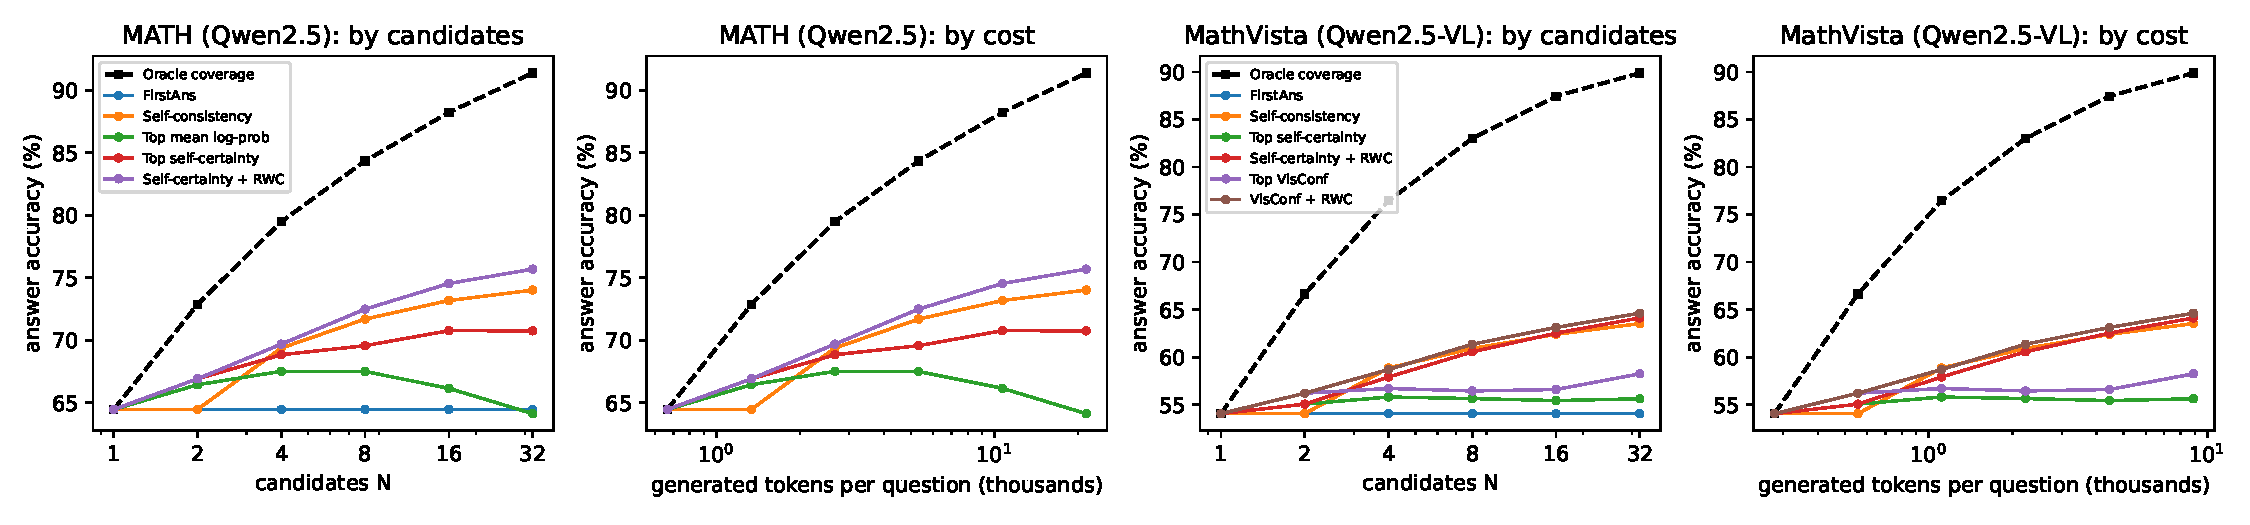
\includegraphics[width=\linewidth]{task3_curves.pdf}
\caption{Held-out answer accuracy and oracle coverage against candidates and generated tokens.}
\label{fig:t3}
\end{figure}

\begin{table}[t]
\centering\footnotesize
\caption{Held-out accuracy (\%) by rule at $N=4,8,32$, with coverage, answer diversity and token cost.}
\label{tab:t3}
\begin{tabular}{lcccccc}
\toprule
 & \multicolumn{3}{c}{MATH} & \multicolumn{3}{c}{MathVista} \\
Rule & 4 & 8 & 32 & 4 & 8 & 32 \\
\midrule
FirstAns & 64.5 & 64.5 & 64.5 & 54.1 & 54.1 & 54.1 \\
Self-consistency & 69.4 & 71.7 & 74.0 & 58.9 & 60.9 & 63.5 \\
Top log-prob & 67.5 & 67.5 & 64.1 & 54.3 & 53.0 & 48.9 \\
Top self-certainty & 68.8 & 69.6 & 70.8 & 55.8 & 55.6 & 55.6 \\
Self-certainty + RWC & 69.7 & 72.5 & 75.7 & 57.9 & 60.6 & 64.1 \\
Shortest (control) & 65.3 & 64.2 & 62.5 & 55.5 & 54.7 & 54.2 \\
Top vision & -- & -- & -- & 55.2 & 54.3 & 54.2 \\
Vision + RWC & -- & -- & -- & 57.6 & 60.5 & 64.0 \\
Top VisConf & -- & -- & -- & 56.7 & 56.5 & 58.2 \\
VisConf + RWC & -- & -- & -- & 58.7 & 61.4 & 64.6 \\
Top tokenwise & -- & -- & -- & 56.5 & 56.1 & 56.8 \\
Tokenwise + RWC & -- & -- & -- & 58.5 & 61.3 & 64.1 \\
\midrule
Oracle coverage & 79.5 & 84.3 & 91.4 & 76.5 & 83.0 & 89.9 \\
Distinct answers & 1.92 & 2.75 & 5.90 & 2.03 & 2.76 & 4.79 \\
Tokens per question & 2,666 & 5,327 & 21,347 & 1,112 & 2,224 & 8,898 \\
\bottomrule
\end{tabular}
\end{table}

\paragraph{Exploration and selection.} Figure~\ref{fig:t3} shows that sampling keeps finding correct answers long after selection stops using them. From $N=1$ to 32, questions with no correct candidate fall from 35.5\% to 8.6\% on MATH and from 45.9\% to 10.1\% on MathVista, yet self-consistency \citep{wang2023selfconsistency} gains only 9.5 points on either. The missed share therefore grows with compute, from 0 to 17.4\% on MATH and 26.3\% on MathVista, and the limit moves from sampling to selection. Returns also fall quickly: the second rollout supplies the first correct answer for 8.4\% of MATH questions, the eighth for 0.8\%, and the last for 0.1\%, while still opening a new answer group 10.2\% of the time. Late samples mostly add wrong alternatives. At $N=2$, self-consistency equals FirstAns because every tie goes to the earlier rollout.

\paragraph{Evidence and consensus.} Table~\ref{tab:t3} isolates the score and the aggregation. On both datasets consensus matters more than the score. Self-consistency beats top self-certainty at $N=32$ by 3.3 points on MATH [0.9, 5.6] and 7.9 on MathVista [4.8, 10.8], and adding RWC to a fixed score gains 4.9 (self-certainty, MATH) and 6.4 (VisConf, MathVista). RWC improves significantly on plain voting only on MATH (+1.7 [0.6, 2.8]). On MathVista, VisConf + RWC is numerically best at 64.6\%, but its advantage over self-consistency (+1.1 [$-$0.3, 2.6]) and self-certainty + RWC (+0.5 [$-$0.8, 1.9]) is not resolved here, which is weaker support than the consistent gains reported by \citet{usman2026visconf} across their models.

\begin{table}[t]
\centering\footnotesize
\caption{Within-question signals at $N=32$ (held-out). Spearman with length, correlation with correctness, and correctness in the top minus bottom score quartile (points).}
\label{tab:t3sig}
\begin{tabular}{llccc}
\toprule
Dataset & Score & $\rho$ length & $r$ correct & Top $-$ bottom [95\% CI] \\
\midrule
MATH & Mean log-prob & +0.22 & +0.144 & +7.9 [+6.4, +9.5] \\
MATH & Self-certainty & -0.16 & +0.221 & +12.0 [+10.5, +13.8] \\
MATH & Shortness & -1.00 & +0.100 & +4.6 [+2.8, +6.2] \\
MathVista & Mean log-prob & +0.33 & +0.034 & +2.0 [+0.4, +3.8] \\
MathVista & Self-certainty & +0.35 & +0.057 & +3.7 [+1.8, +5.3] \\
MathVista & Shortness & -1.00 & +0.079 & +3.7 [+2.0, +5.4] \\
MathVista & Vision share & -0.69 & +0.045 & +3.6 [+1.8, +5.3] \\
MathVista & VisConf & -0.28 & +0.098 & +7.3 [+5.4, +9.2] \\
MathVista & Tokenwise & -0.32 & +0.090 & +7.2 [+5.4, +9.1] \\
\bottomrule
\end{tabular}
\end{table}

The most useful negative result is mean log-probability. On MATH it helps at first (about 3 points at $N=4$ and 8) and then declines to the level of FirstAns ($-$0.3 [$-$2.4, 1.7]); on MathVista it never clearly helps and ends 5.2 points below FirstAns [$-$7.7, $-$2.6]. What it selects suggests why: at $N=32$ it returns a capped rollout 14.5\% of the time on MATH and 17.9\% on MathVista, against base rates of 1.7\% and 1.5\%. Likely reason: repetition loops are easy to predict, so they score well, and larger pools are more likely to contain one. Self-certainty largely avoids this (0.2\% capped on MATH). Table~\ref{tab:t3sig} shows other confounds. Shortness alone separates quartiles by 4.6 and 3.7 points, about as well as self-certainty on MathVista. Vision share correlates at $-$0.69 with length, as attention moves towards generated tokens in longer outputs, so raw vision share partly measures brevity. Confidence and vision are also negatively related within a rollout (mean $r=-0.21$, positive for only 11\% of questions). Nevertheless, multiplying them gives the strongest MathVista signal, a 7.3-point quartile gap against 3.7 and 3.6 for its parts. Tokenwise fusion differs from VisConf by a covariance, which we verified numerically (error $5\times10^{-17}$), and adds nothing: $-$1.5 [$-$3.5, 0.4] with top selection and $-$0.5 [$-$1.3, 0.3] with RWC. The trajectories in Appendix~\ref{app:t3} show no consistent separation of right and wrong rollouts token by token. None of this shows that attention causes correct answers.

\begin{table}[t]
\centering\footnotesize
\caption{Live results on 50 MATH questions: accuracy (\%), mean output and input tokens and seconds per question, truncated calls and failed extractions. Initial is the first parallel response, shared with refinement.}
\label{tab:live}
\begin{tabular}{lcccccc}
\toprule
Strategy & Accuracy & Output tokens & Input tokens & Seconds & Truncated & No extraction \\
\midrule
Single long & \pend{--} & \pend{--} & \pend{--} & \pend{--} & \pend{--} & \pend{--} \\
Parallel + vote & \pend{--} & \pend{--} & \pend{--} & \pend{--} & \pend{--} & \pend{--} \\
Refinement & \pend{--} & \pend{--} & \pend{--} & \pend{--} & \pend{--} & \pend{--} \\
Initial only & \pend{--} & \pend{--} & \pend{--} & \pend{--} & \pend{--} & \pend{--} \\
\bottomrule
\end{tabular}
\end{table}

\begin{table}[t]
\centering\footnotesize
\caption{Stopping on held-out questions. Settings ($\tau$, or $\tau,\gamma$) chosen on development only. Stop \%: share stopping at $n=4/8/16/32$.}
\label{tab:adaptive}
\begin{tabular}{llccccc}
\toprule
Dataset & Policy & Setting & Accuracy (\%) & Tokens per question & Mean rollouts & Stop \% \\
\midrule
MATH & Fixed $N=16$ & -- & 73.2 & 10,667 & 16 & -- \\
MATH & Fixed $N=32$ & -- & 74.0 & 21,347 & 32 & -- \\
MATH & Agreement & 0.625 & 73.8 & 10,187 & 11.9 & 67 / 5 / 1 / 27 \\
MATH & Quality-aware & 0.5, 0.25 & 73.7 & 8,574 & 10.1 & 72 / 6 / 2 / 20 \\
MathVista & Fixed $N=16$ & -- & 62.4 & 4,447 & 16 & -- \\
MathVista & Fixed $N=32$ & -- & 63.5 & 8,898 & 32 & -- \\
MathVista & Agreement & 0.625 & 63.6 & 4,508 & 13.3 & 58 / 9 / 2 / 31 \\
MathVista & Quality-aware & 0.5, 0 & 63.0 & 3,363 & 10.1 & 68 / 10 / 3 / 19 \\
\bottomrule
\end{tabular}
\end{table}

\paragraph{Breadth and refinement.} On the fixed 50 MATH questions, with the same 3,072-token allowance, Table~\ref{tab:live} compares one long response, three independent samples with voting, and critique-and-revision \citep{madaan2023selfrefine} of the first sample. One long response and refinement both reach 62\% and parallel voting 54\%, but with 50 questions no difference is resolved: parallel against long is $-$8 [$-$20, 6] and refinement against parallel +8 [0, 18]. An equal allowance is not an equal cost. Long responses rarely need their budget (760 output tokens on average, 2 of 50 calls capped), whereas a third of the allowance is often too short for a sample: 25 of 150 parallel calls stop at 1,024 tokens, and 11 of the 50 votes return no answer under the offline rule. Voting over extracted answers only raises parallel to 58\%, so truncation accounts for about half of its deficit. Parallel is also the slowest, at 1,857 output tokens and 99\,s per question against 41\,s; refinement takes 66\,s and reads an 890-token prompt that contains the first attempt. Revision never turned a correct answer wrong, and all 3 of its wrong-to-correct cases (+6 [0, 14] over the initial sample) are first attempts that were cut off before an answer. It changed 10 answers, all of them missing ones, and never revised an answer that had been extracted, so here it acts as a continuation of truncated work rather than a correction of errors.

\paragraph{Adaptive allocation.} Table~\ref{tab:adaptive} and Figure~\ref{fig:t3adapt} show that observed agreement is an effective guide to stopping. The agreement rule selected on development ($\tau=0.625$) saves 52\% of tokens on MATH and 49\% on MathVista relative to fixed-32, with accuracy differences of $-$0.25 [$-$0.61, 0.10] and +0.05 [$-$0.51, 0.71]. At similar cost it beats fixed $N=16$ on MathVista (+1.2 [0.4, 2.0]) and is not distinguishable from it on MATH (+0.6 [$-$0.05, 1.2]). Quality-aware stopping saves more (60\% and 62\%) by accepting a lower agreement threshold, with a greater accuracy cost that remains within interval ($-$0.35 and $-$0.50). The policy spends effort where it can help: questions whose entire pool is correct stop at 4 rollouts, whereas MATH questions with some but at most a quarter correct use 25.8 on average. Its main weakness is confident agreement on wrong answers: 25\% of MATH and 20\% of MathVista questions with no correct rollout at all still stop at $n=4$. Only a small part of the damage from stopping early is recoverable, however. Wrong early stops occur in 8.2\% and 14.1\% of runs, but fixed-32 would have been right in just 0.7\% and 1.6\% of runs (about a tenth of those stops), which is why accuracy barely moves. Pool fractions here are retrospective and played no part in any decision. These are offline simulations that count generated tokens; a real deployment also pays for scoring and for attention collection.

\begin{figure}[t]
\centering
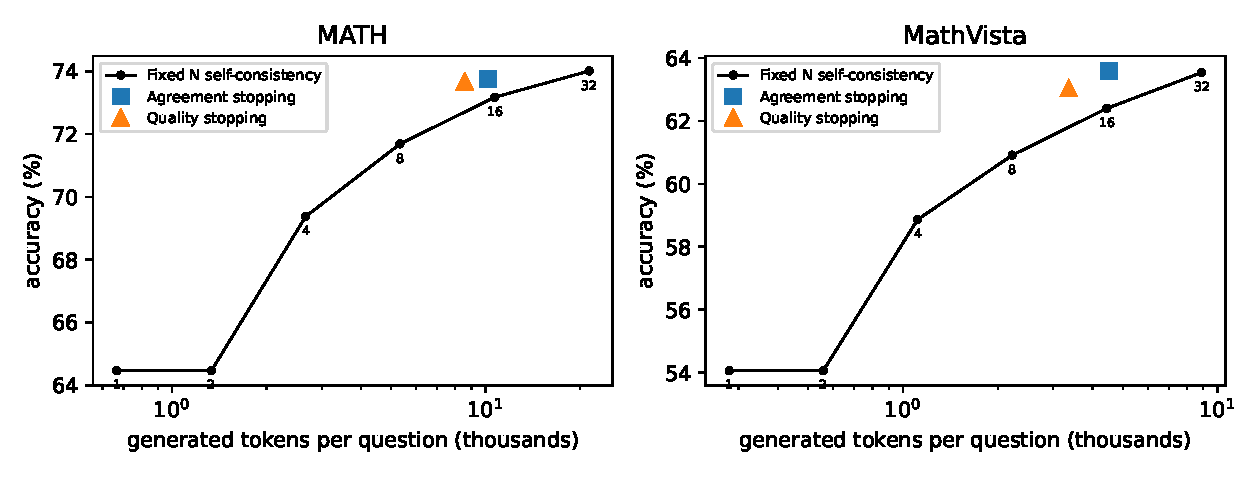
\includegraphics[width=0.68\linewidth]{task3_adaptive.pdf}
\caption{Selected stopping policies against fixed-$N$ self-consistency on the held-out questions.}
\label{fig:t3adapt}
\end{figure}

\paragraph{Compute and reliability.} The stopping policies give the best trade-offs we measured: agreement stays closest to fixed-32 and quality-aware is cheapest, though we did not test them directly against each other. RWC is a cheap addition once scores exist. Two reliability points follow from the failures above: score-only selection is not safe without a guard against capped outputs, and no internal signal here identifies a question whose rollouts agree on a wrong answer. Results compare two model-dataset pairs and do not isolate the effect of adding vision. \citet{usman2026visconf} and our run also differ in splits and scoring, so the gap in VisConf's advantage may have several causes.

\section{Conclusion}
The three experiments share a pattern: the headline metric rarely tells the whole story. All fine-tuning methods gain on mathematics, and apart from L2-SP's lead over LoRA-4 their clearest differences are in bias, repetition and cost; OPLoRA's exact geometric guarantee shows no measurable behavioral gain at these update sizes. A small connector and adapters produce real image dependence, strong on presence and weaker on counting and natural questions. And extra samples soon add more candidates than a selection rule can use, so agreement-based stopping recovers most of the benefit at half the cost; in the live run, revision helped only by finishing truncated first attempts. All results use one seed per configuration, and the smaller test sets limit how small a difference we could detect.

\small
\bibliographystyle{plainnat}
\bibliography{references}
\normalsize

\appendix
\section{Task 2 breakdown by question type}\label{app:t2}
\begin{table}[H]
\centering\footnotesize
\caption{Test accuracy (\%) by question type for the 196-token model, with the correct-minus-complementary advantage.}
\begin{tabular}{lcccccc}
\toprule
Type & Pairs & Correct & Compl. & Mismatched & None & Correct $-$ compl. \\
\midrule
Presence & 32 & 95.3 & 4.7 & 43.8 & 50.0 & +90.6 [+78.1, +100.0] \\
Counting & 32 & 43.8 & 17.2 & 21.9 & 25.0 & +26.6 [+12.5, +40.6] \\
Yes/no & 36 & 63.9 & 45.7 & 55.6 & 45.4 & +18.2 [+1.9, +34.4] \\
Number & 24 & 36.5 & 20.0 & 22.5 & 21.2 & +16.5 [+3.1, +31.2] \\
Other & 36 & 46.1 & 16.0 & 13.7 & 14.7 & +30.1 [+15.3, +46.8] \\
\bottomrule
\end{tabular}
\end{table}

\section{Task 3 additional evidence}\label{app:t3}
\begin{table}[H]
\centering\footnotesize
\caption{Failure decomposition on held-out questions (\% of questions): no correct candidate generated, and correct candidate generated but missed.}
\begin{tabular}{lcccc}
\toprule
Dataset & $N$ & Not generated & Missed (self-consistency) & Missed (quality + RWC) \\
\midrule
MATH & 1 & 35.5 & 0.0 & 0.0 \\
MATH & 4 & 20.5 & 10.1 & 9.8 \\
MATH & 32 & 8.6 & 17.4 & 15.7 \\
MathVista & 1 & 45.9 & 0.0 & 0.0 \\
MathVista & 4 & 23.5 & 17.6 & 17.8 \\
MathVista & 32 & 10.1 & 26.3 & 25.2 \\
\bottomrule
\end{tabular}
\end{table}

\begin{figure}[H]
\centering
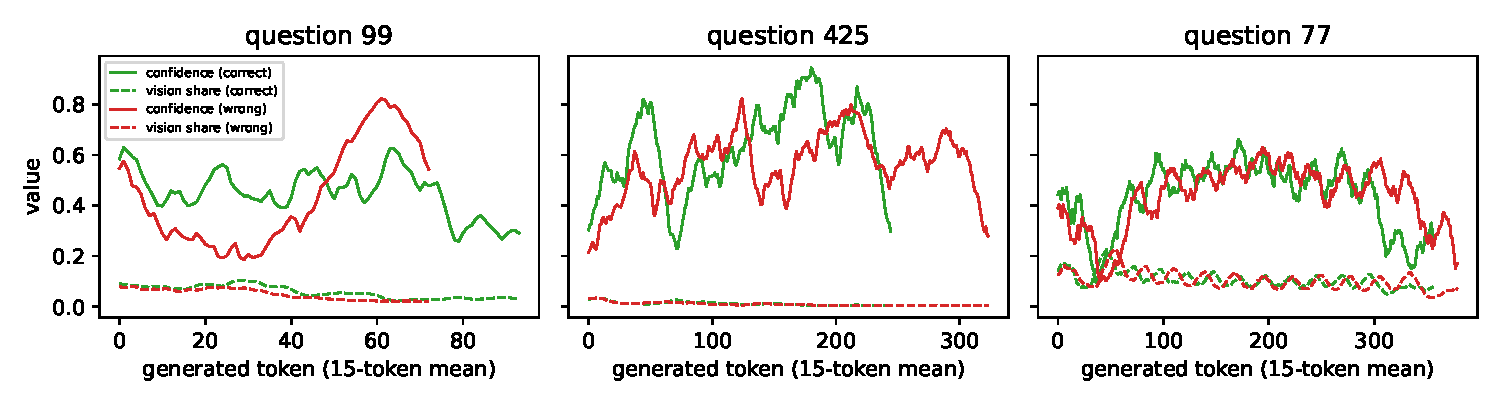
\includegraphics[width=\linewidth]{task3_trajectories.pdf}
\caption{Calibrated confidence and vision share for one correct and one wrong rollout. Rule: the first three held-out MathVista questions, in split order, with both right and wrong rollouts of 50 to 400 tokens; the lowest-numbered of each.}
\end{figure}

\paragraph{Representative cases.} Each was picked by a fixed rule: shuffle held-out questions with seed 6304, use the first candidate order, and take the first two of each kind (\texttt{results/task3/*/cases.json}). \emph{Consensus right, score wrong}: MATH \texttt{test:3472}, where half the pool says 621 and top self-certainty returns 223. \emph{Score right, consensus wrong}: MATH \texttt{test:2755}, where the correct remainder $17x-13$ appears in 22\% of rollouts, but the vote returns 4 while self-certainty and RWC both find it. \emph{Missed by all}: MathVista 598, with 6\% of rollouts correct. \emph{Premature stop}: MATH \texttt{test:4281} stops at $n=4$ with 75\% support on a wrong answer, though 44\% of the pool is correct and fixed-32 recovers it in that order. \emph{Refinement} (live run, the first wrong-to-correct case in question order): for the least multiple of 72 with exactly 16 factors (\texttt{test:3504}, answer 216), the first sample works through the factorizations of 16 case by case and reaches the 1,024-token cap before giving an answer. The revision repeats the same case analysis, finishes it and returns $\boxed{216}$ in 1,080 tokens. The single long response also solves it, while two of the three parallel samples hit the cap and the vote returns no answer.

\paragraph{Deviations and choices.} Some MathVista extractions carry units or LaTeX (\texttt{14.63 \textbackslash, \textbackslash text\{m/s\}}), so we strip these before applying the benchmark's numeric rules. All steps ran as prescribed otherwise. GPU runs used a T4 rather than a larger accelerator. The scorer was tested on development questions only and then frozen.

\end{document}
